\documentclass[twocolumn]{article}

\usepackage{graphicx}

\newcommand{\size}{.85}

\title{Homework}
\author{Mark Royer}
\date{}

\begin{document}

\maketitle

This document is meant to be an example of the type of discussion I am
looking for in \texttt{results.pdf}.  In general, I expect to see the
results of your program plotted with theoretical results.  To give you
a more concrete example, I have performed the tests on
\texttt{quickSort}. You are expected to perform the tests on
\texttt{bubbleSort}, \texttt{insertionSort}, \texttt{mergeSort}, and
\texttt{selectionSort}.  A short summary of the data will
suffice; no additional statistical analysis is required.


\section*{Quick Sort}

This section describes the test results of the
\texttt{quickSort} routine run on data in ascending, descending, and random
order. According to the theoretical results, quick sort is $O(n^2)$ in the
worst case and $\Omega(n\log n)$ in the best case.  On average, quick
sort should be $O(n\log n)$.

The algorithm uses the first element as the partition element.  When
the given data is already sorted in ascending or descending order,
quick sort degenerates into a form of selection sort, which is
$O(n^2)$.  Figures \ref{asc} and \ref{desc} show the results of
sorting data that is in ascending and descending order plotted with the function
$n^2$. As expected, the resulting curve looks quadratic.

\begin{figure}[h]
 \centerline{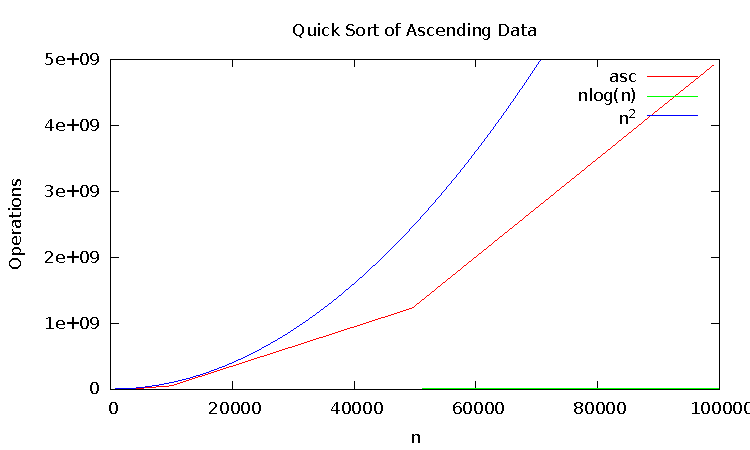
\includegraphics[width=\size\columnwidth]{qsasc}}
 \caption{Data in ascending order.}\label{asc}
\end{figure}

\begin{figure}[h]
 \centerline{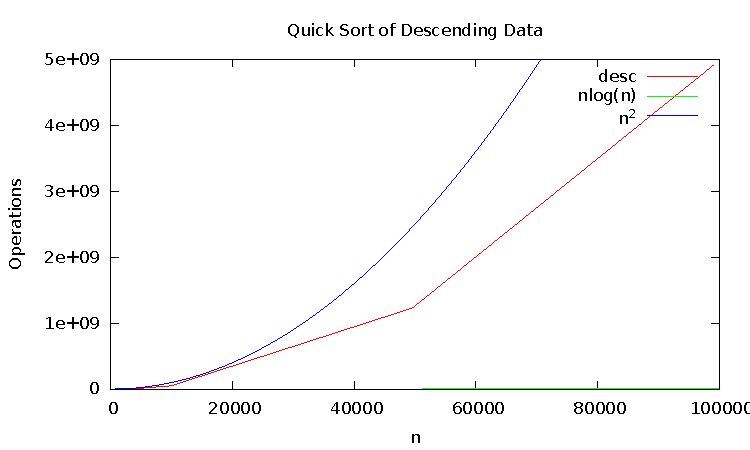
\includegraphics[width=\size\columnwidth]{qsdesc}}
 \caption{Data in descending order.}\label{desc}
\end{figure}

When quick sort picks the perfect partition element, the sorting
routine begins to behave like a form of merge sort.  If the input data
is random, we would expect the chosen pivot element to be good
sometimes and bad sometimes, but on average, not too bad.  From this,
we would conclude that on random data, quick sort should perform
closer to $O(n\log n)$.  Figure \ref{random} shows the results of
sorting random data with functions $n^2$ and $n\log n$. As expected,
the results look $O(n\log n)$.

\begin{figure}[h]
 \centerline{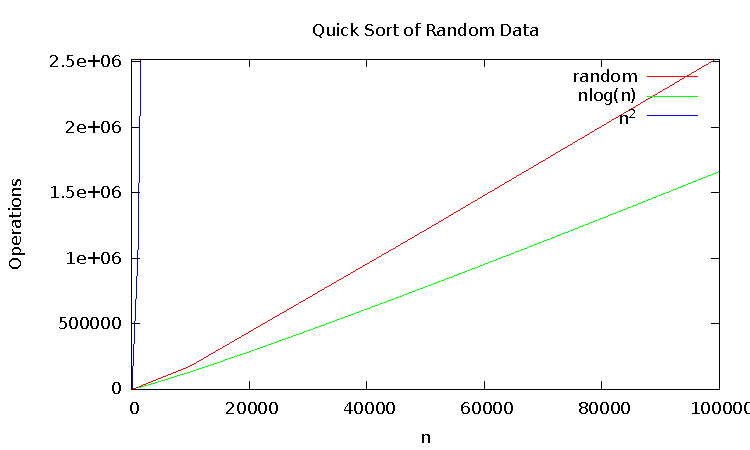
\includegraphics[width=\size\columnwidth]{qsrandom}}
 \caption{Data in random order.}\label{random}
\end{figure}


\end{document}


